\documentclass[twoside,12pt,openright]{report}

% ======================================================================
%  TIET report layout (built in, so no external tietreport.cls is needed)
% ======================================================================
\makeatletter
%% ===================================================
%% Geometry: Page margins and asymmetric layout
%% ===================================================
%% Configure margins for two-sided printing.
%% Inner margin (binding edge) is wider for gutter;
%% outer margins are narrower. Top/bottom margins
%% accommodate headers/footers and content balance.
\usepackage[
  inner=1.5in,
  outer=1in,
  top=1.8in,
  bottom=0.85in
]{geometry}

%% ===================================================
%% Fancyhdr: Alternating headers with page numbers
%% ===================================================
%% Left (even) pages: page number + title header.
%% Right (odd) pages: project title + page number.
%% Both placed on outer margin for binding edge
%% clarity. Footer empty to maximize text area.
%% Header rule (0.5pt) provides visual separation.
\usepackage{fancyhdr}
\pagestyle{fancy}
\fancyhf{}
\fancyhead[LE]{\thepage \quad \@tpHeader}
\fancyhead[RO]{\@tpTitle \quad \thepage}
\renewcommand{\headrulewidth}{0.5pt}
\renewcommand{\footrulewidth}{0pt}

%% ===================================================
%% Titlesec: Custom chapter title formatting
%% ===================================================
%% Chapter titles use raggedleft (right-aligned)
%% with bold/large label, followed by huge title
%% and horizontal rule. Spacing optimized for
%% visual hierarchy. Chapter opening pages use
%% empty style (no headers).
\usepackage{titlesec}
\titleformat{\chapter}[display]
  {\raggedleft\bfseries\large}
  {Chapter \thechapter}
  {0.3em}
  {\huge}
  [\vspace{0.1em}\hrule]
\titlespacing*{\chapter}{0pt}{-50pt}{40pt}
\assignpagestyle{\chapter}{empty}

%% ===================================================
%% Required packages: Hyperref, graphics, math
%% ===================================================
%% Standard packages for links, images, and
%% mathematical notation support.
\usepackage{hyperref}
\usepackage{graphicx}
\usepackage{amsmath}
\usepackage{amssymb}

%% ===================================================
%% Internal Variables: Title page content storage
%% ===================================================
%% Prefix @tp denotes "title page" internal vars.
%% These hold configuration set via public commands
%% below. Users should not access these directly.

%% Title page header (e.g., course code and lab)
\newcommand{\@tpHeader}{%
  UCS 503 Software Engineering Project Report%
}

%% Main project title
\newcommand{\@tpTitle}{Proposal to Final}

%% Project subtitle/description
\newcommand{\@tpSubTitle}{%
  How to Write a Project Report%
}

%% Author list (4 students with roll numbers)
\newcommand{\@tpAuthors}{%
  \texttt{102XXXXXXX} {Name Title} \\
  \texttt{102XXXXXXX} {Name Title} \\
  \texttt{102XXXXXXX} {Name Title} \\
  \texttt{102XXXXXXX} {Name Title}%
}

%% Degree, year, group info below authors
\newcommand{\@tpSubText}{%
  Group: \texttt{3XXX} BE Third Year, CSE%
}

%% Faculty advisor/guide name
\newcommand{\@tpAdvisor}{%
  Dr. NAME OF THE ADVISOR%
}

%% Footer: evaluation period, department, institution
\newcommand{\@tpFooter}{%
  \large Mid-Semester Evaluation \\[0.2cm]
  \bfseries Computer Science and Engineering%
  \\ Department \\[0.15cm]
  Thapar Institute of Engineering and%
  \\ Technology, Patiala%
}

%% ===================================================
%% Public Commands: User-facing configuration
%% ===================================================
%% Call these in preamble to customize title page.
%% Example: \TitlePageHeader{CS 504 Lab}

%% Set title page header
\newcommand{\TitlePageHeader}[1]{%
  \renewcommand{\@tpHeader}{#1}%
}

%% Set main project title
\newcommand{\ProjectTitle}[1]{%
  \renewcommand{\@tpTitle}{#1}%
}

%% Set project subtitle
\newcommand{\ProjectSubTitle}[1]{%
  \renewcommand{\@tpSubTitle}{#1}%
}

%% Set author list (override default)
\renewcommand{\author}[1]{%
  \renewcommand{\@tpAuthors}{#1}%
}

%% Set degree/year/group info
\newcommand{\TitlePageSubText}[1]{%
  \renewcommand{\@tpSubText}{#1}%
}

%% Set advisor name
\newcommand{\AdvisorName}[1]{%
  \renewcommand{\@tpAdvisor}{#1}%
}

%% Set footer text (evaluation period, dept, etc)
\newcommand{\TitlePageFooterText}[1]{%
  \renewcommand{\@tpFooter}{#1}%
}

%% ===================================================
%% Maketitle: Render custom title page
%% ===================================================
%% Override \maketitle to produce styled title page
%% using configured variables. Centered layout with
%% institutional branding. After title page, a blank
%% page follows (ready for TOC on next page).

\renewcommand{\maketitle}{%
  \begin{titlepage}
    \thispagestyle{empty}
    \centering
    \vspace*{0.5cm}

    {\large \textbf{\@tpHeader}}

    \vspace{2cm}
    {\LARGE \textbf{\@tpTitle}}

    \vspace{0.2cm}
    {\@tpSubTitle}

    \vspace{3.5cm}
    {\large \textbf{Submitted by:}}

    \vspace{0.2cm}
    {\large \@tpAuthors}

    \vspace{0.5cm}
    {\normalsize \@tpSubText}

    \vfill

    {\large \textbf{Submitted to:}}

    \vspace{0.2cm}
    {\normalsize \@tpAdvisor}

    \vspace{2cm}
    {\normalsize \@tpFooter}
  \end{titlepage}

  \newpage
  \thispagestyle{empty}%
}
\makeatother



% Import images
\usepackage{graphicx}

% Extra packages required by the report content
\usepackage{float}
\usepackage{tabularx}
\usepackage{xcolor}
\usepackage{listings}
\usepackage{adjustbox}
\usepackage{needspace}
\usepackage{tikz}
\usetikzlibrary{arrows.meta,positioning,shapes.geometric,fit,calc}



%% ==================================================
%% CODE LISTING AND DIAGRAM STYLES
%% ==================================================

\lstdefinestyle{code}{
  basicstyle=\ttfamily\scriptsize,
  keywordstyle=\bfseries,
  commentstyle=\color{gray}\itshape,
  numbers=left, numberstyle=\tiny\color{gray}, numbersep=5pt,
  frame=single, rulecolor=\color{gray!60},
  backgroundcolor=\color{gray!6},
  breaklines=true, tabsize=2, showstringspaces=false,
  xleftmargin=1.2em, aboveskip=4pt, belowskip=2pt
}
\lstdefinelanguage{json}{
  string=[b]", morekeywords={true,false}, sensitive=true
}

\tikzset{
  >=Stealth,
  blk/.style={rectangle,rounded corners=3pt,draw=black,fill=white,thick,
              minimum height=1.2cm,text width=2.3cm,align=center,font=\small},
  fl/.style={font=\scriptsize,align=center}
}

% ground symbol: \gnd{coordinate}
\newcommand{\gnd}[1]{%
  \draw[thick] (#1) -- ++(0,-0.3) coordinate (g);
  \draw[thick] ($(g)+(-0.25,0)$) -- ($(g)+(0.25,0)$);
  \draw[thick] ($(g)+(-0.16,-0.08)$) -- ($(g)+(0.16,-0.08)$);
  \draw[thick] ($(g)+(-0.07,-0.16)$) -- ($(g)+(0.07,-0.16)$);}

% UML stick-figure actor: \actor{x}{y}{label}
\newcommand{\actor}[3]{%
  \begin{scope}[shift={(#1,#2)}]
    \draw[thick] (0,0.55) circle (0.17);
    \draw[thick] (0,0.38)--(0,-0.1) (-0.3,0.25)--(0.3,0.25)
                 (0,-0.1)--(-0.25,-0.5) (0,-0.1)--(0.25,-0.5);
    \node[font=\footnotesize,align=center,below] at (0,-0.5) {#3};
  \end{scope}}

% Scale a diagram down only if it is wider/taller than the page allows
\newcommand{\fitfig}[2][0.27]{\begin{adjustbox}{max width=\linewidth,max height=#1\textheight,center}#2\end{adjustbox}}

%% ==================================================
%% CUSTOMIZE THESE FIELDS FOR YOUR PROJECT
%% ==================================================

% Course/Lab header
\TitlePageHeader{%
  UCS 503 - Software Engineering%
}

% Main project title
\ProjectTitle{%
  Real-Time Library Seat Occupancy Management System%
}

% Subtitle or project description
\ProjectSubTitle{%
  An IoT-Based Live Seat Availability System%
}

% Student information (up to 4 students)
\author{%
  \texttt{1024031135} Saksham Kansal \\
  \texttt{1024031118} Ishaan Gupta \\
  \texttt{1024031137} Sanshi%
}

% Group number, degree, year, program
\TitlePageSubText{%
  Computer Engineering Department (COE)%
}

% Faculty advisor/guide name
\AdvisorName{%
  Ms. Jhonsy Bansal%
}

% Evaluation period and department info
\TitlePageFooterText{{%
    \large August 2026 \\[0.2cm]
    \bfseries Computer Engineering
    Department%
  } \\[0.15cm]
  Thapar Institute of Engineering and Technology,
  Patiala%
}

%% ==================================================

\begin{document}

% Stop twoside's \flushbottom from stretching list/heading spacing on partly filled pages
\raggedbottom

% Compact layout: start chapters on the next page instead of the next
% right-hand page (removes blank pages). Delete this line to restore openright.
\makeatletter\@openrightfalse\makeatother

% Generate title page
\maketitle

% Table of contents (auto-generated from chapters)
\tableofcontents

% ===== CHAPTER 1: INTRODUCTION =====

\chapter{Introduction}

\section{Background and Context}

University libraries are among the most heavily used shared spaces on a campus, and demand
peaks sharply around examinations and assignment deadlines. At such times students must
physically walk through reading halls to discover where a seat is available. Conventional
gate counters report how many people are inside the building, but not \emph{where} the free
seats are. The result is wasted search time, continuous hallway movement and noise that
disturbs students who are already studying.

Low-cost Wi-Fi microcontrollers, proximity sensors and managed real-time cloud databases now make it feasible to monitor every seat and publish its state to any phone or display within a fraction of a second.

\subsection{Problem Statement}
\label{sec:problem}

The current way of locating a study seat has three shortcomings, summarised in
Table~\ref{tab:problems}.

\begin{table}[H]
\centering
\small
\renewcommand{\arraystretch}{1.15}
\begin{tabular}{|p{0.2\linewidth}|p{0.43\linewidth}|p{0.26\linewidth}|}
  \hline
  \textbf{Problem} & \textbf{Description} & \textbf{Operational need} \\
  \hline
  Manual fragmentation &
  Students must physically navigate multiple floors and aisles during peak hours, causing
  hallway noise and wasted search time. &
  Remote, instant knowledge of free seats before walking to the hall. \\
  \hline
  Low transparency &
  Static headcount boards at library gates give lagging aggregate metrics without showing
  desk-level availability. &
  Seat-level visibility rather than a single building-wide count. \\
  \hline
  Administrative blindspot &
  Staff lack real-time and historical analytics to balance traffic across reading halls or
  to optimise HVAC and facility allocation. &
  Live and historical utilisation analytics for facility planning. \\
  \hline
\end{tabular}
\caption{Core problems and the corresponding operational need}
\label{tab:problems}
\end{table}

\section{Project Objectives}

\begin{enumerate}
  \item \textbf{Detection:} Detect physical presence at every monitored study seat using
    low-cost IR sensors.
  \item \textbf{Noise filtering:} Filter sensor noise so that momentary obstructions do not
    change a seat's state.
  \item \textbf{Transmission:} Transmit seat states to the cloud over Wi-Fi with minimal
    latency.
  \item \textbf{Student view:} Present a live seat map and capacity metrics on mobile browsers
    and on an entrance kiosk display.
  \item \textbf{Admin view:} Give administrators an analytics dashboard for utilisation,
    session time and peak-hour monitoring.
\end{enumerate}

\subsection{Scope and Organisation of the Report}

The system covers sensing, communication, cloud synchronisation and presentation for study
seats in a library zone. It identifies only whether a seat is occupied; it does not capture
images, identify individuals or enforce seat reservations. The prototype demonstrates the
complete data path from a sensor to a browser, and the design scales to additional seats and
zones by adding sensor nodes and database branches.

Chapter~\ref{ch:method} covers the requirements, architecture, UML models and implementation;
Chapter~\ref{ch:results} gives the test plan, discussion and limitations; and
Chapter~\ref{ch:concl} concludes with future scope.

% ===== CHAPTER 2: METHODOLOGY & DESIGN =====

\chapter{Methodology and Design}
\label{ch:method}

\section{Requirements Analysis}

\subsection{Stakeholders}

\begin{itemize}
  \item \textbf{Students:} Need to know which seats are free and how full the library is
    before and while travelling to it.
  \item \textbf{Library staff / administrators:} Need live occupancy and historical analytics
    for traffic balancing and facility allocation.
  \item \textbf{Sensor node (system actor):} Continuously senses seats and publishes state.
\end{itemize}

\subsection{Functional Requirements}

\begin{table}[H]
\centering
\small
\renewcommand{\arraystretch}{1.1}
\begin{tabularx}{\linewidth}{|l|X|}
  \hline
  \textbf{ID} & \textbf{Requirement} \\
  \hline
  FR1 & Detect the presence of a person at each monitored seat using an active IR sensor. \\
  \hline
  FR2 & Apply a 3-second software debounce window before a seat changes state. \\
  \hline
  FR3 & The ESP32 node encodes binary seat states into a JSON payload and sends it over Wi-Fi
        to the cloud database. \\
  \hline
  FR4 & The cloud database keeps a synchronised state tree and notifies clients of changes
        without manual refresh. \\
  \hline
  FR5 & The student dashboard shows a floor map: vacant seats green, occupied seats red. \\
  \hline
  FR6 & The dashboards show total, occupied and available seats and the occupancy rate. \\
  \hline
  FR7 & The entrance kiosk displays live capacity and availability for the zone. \\
  \hline
  FR8 & The administrator dashboard shows average session time, peak hour, weekly trend,
        hourly peak distribution and the occupied/available split. \\
  \hline
\end{tabularx}
\caption{Functional requirements}
\label{tab:fr}
\end{table}

\subsection{Non-Functional Requirements}

\begin{table}[H]
\centering
\small
\renewcommand{\arraystretch}{1.1}
\begin{tabularx}{\linewidth}{|l|l|X|}
  \hline
  \textbf{ID} & \textbf{Attribute} & \textbf{Requirement} \\
  \hline
  NFR1 & Performance & Sub-second cloud-to-client synchronisation (excluding the deliberate
                       3-s debounce). \\
  \hline
  NFR2 & Reliability & Momentary obstructions must not cause flickering of seat colours. \\
  \hline
  NFR3 & Usability   & The student interface is responsive and usable on a mobile browser. \\
  \hline
  NFR4 & Scalability & Seats and zones can be added without redesigning the data model. \\
  \hline
  NFR5 & Cost        & Inexpensive off-the-shelf sensing hardware. \\
  \hline
  NFR6 & Privacy     & No images or personal identifiers; only a binary presence state is
                       recorded. \\
  \hline
\end{tabularx}
\caption{Non-functional requirements}
\label{tab:nfr}
\end{table}

\section{System Architecture}

\subsection{High-Level Design}

The system is organised in three layers, shown in Figure~\ref{fig:arch}: an \emph{edge layer}
that senses and encodes seat state, a \emph{cloud layer} that stores and distributes it, and a
\emph{presentation layer} that renders it for students and staff.

\begin{figure}[H]
\centering
\fitfig{%
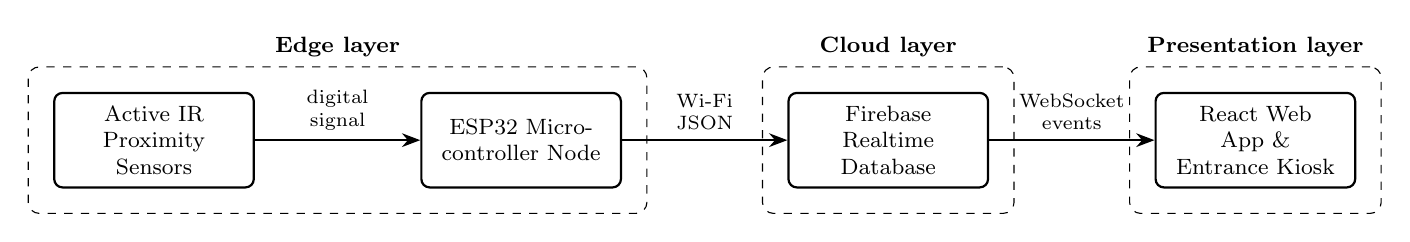
\begin{tikzpicture}[node distance=2.1cm,blk/.append style={text width=2.3cm,font=\footnotesize}]
  \node[blk] (ir)  {Active IR\\Proximity Sensors};
  \node[blk,right=of ir]  (esp) {ESP32 Micro-controller Node};
  \node[blk,right=of esp] (fb)  {Firebase\\Realtime Database};
  \node[blk,right=of fb]  (web) {React Web App \&\\Entrance Kiosk};
  \draw[->,thick] (ir)  -- node[fl,above]{digital\\signal} (esp);
  \draw[->,thick] (esp) -- node[fl,above]{Wi-Fi\\JSON} (fb);
  \draw[->,thick] (fb)  -- node[fl,above]{WebSocket\\events} (web);
  \node[draw=black,dashed,rounded corners,fit=(ir)(esp),inner sep=9pt,
        label={[font=\footnotesize\bfseries,text=black]above:Edge layer}] {};
  \node[draw=black,dashed,rounded corners,fit=(fb),inner sep=9pt,
        label={[font=\footnotesize\bfseries,text=black]above:Cloud layer}] {};
  \node[draw=black,dashed,rounded corners,fit=(web),inner sep=9pt,
        label={[font=\footnotesize\bfseries,text=black]above:Presentation layer}] {};
\end{tikzpicture}}
\caption{End-to-end system architecture}
\label{fig:arch}
\end{figure}

Active IR sensors on the seats feed an ESP32 node~\cite{esp32}, which publishes debounced seat states as JSON over Wi-Fi to a Firebase Realtime Database~\cite{firebase}; the database pushes WebSocket events to the React web application and entrance kiosk~\cite{react}.

\subsection{Seating Layout}

Figure~\ref{fig:seating} shows the physical arrangement. Each seat has an IR sensor mounted
at the table edge facing the chair, wired to a central controller that connects to an ESP32
Wi-Fi node. Here a vacant seat is drawn white and an occupied seat dark; the web dashboards
show green and red.

\begin{figure}[H]
\centering
\fitfig{%
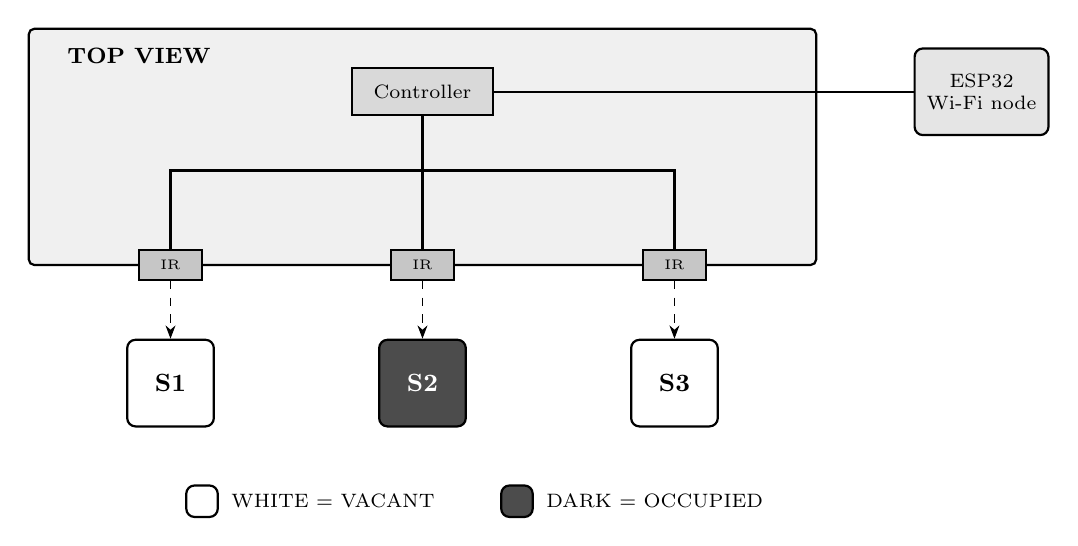
\begin{tikzpicture}[
  seat/.style={draw=black,fill=#1,thick,rounded corners=3pt,minimum size=1.1cm,font=\small\bfseries},
  irn/.style={draw,thick,fill=gray!45,minimum width=0.8cm,minimum height=0.38cm,font=\tiny}]
  \draw[thick,fill=gray!12,rounded corners=2pt] (0,0) rectangle (10,3);
  \node[font=\footnotesize\bfseries] at (1.4,2.65) {TOP VIEW};
  \node[draw,thick,fill=gray!30,minimum width=1.8cm,minimum height=0.6cm,font=\scriptsize] (ctl) at (5,2.2) {Controller};
  \foreach \x/\n in {1.8/1,5/2,8.2/3}{
    \node[irn] (ir\n) at (\x,0) {IR};
  }
  \coordinate (j) at (5,1.2);
  \draw[thick] (ctl.south) -- (j);
  \draw[thick] (j) -| (ir1.north);
  \draw[thick] (j) -- (ir2.north);
  \draw[thick] (j) -| (ir3.north);
  \node[seat=white] (c1) at (1.8,-1.5) {S1};
  \node[seat=black!70,text=white] (c2) at (5.0,-1.5) {S2};
  \node[seat=white] (c3) at (8.2,-1.5) {S3};
  \foreach \n in {1,2,3}{ \draw[dashed,->] (ir\n.south) -- (c\n.north); }
  \node[draw,thick,fill=gray!20,rounded corners=3pt,minimum width=1.7cm,minimum height=1.1cm,
        font=\scriptsize,align=center] (wifi) at (12.1,2.2) {ESP32\\Wi-Fi node};
  \draw[thick] (ctl.east) -- (wifi.west);
  \node[seat=white,minimum size=0.4cm] at (2.2,-3.0) {};
  \node[font=\scriptsize,right] at (2.45,-3.0) {WHITE = VACANT};
  \node[seat=black!70,minimum size=0.4cm] at (6.2,-3.0) {};
  \node[font=\scriptsize,right] at (6.45,-3.0) {DARK = OCCUPIED};
\end{tikzpicture}}
\caption{Seating layout (top view): per-seat IR sensors wired to a controller and an ESP32 node}
\label{fig:seating}
\end{figure}

\subsection{Hardware Design}

\begin{table}[H]
\centering
\small
\renewcommand{\arraystretch}{1.1}
\begin{tabularx}{\linewidth}{|l|X|}
  \hline
  \textbf{Component} & \textbf{Role} \\
  \hline
  ESP32 development board & Reads the GPIO inputs, runs the debounce logic, builds JSON
    payloads and connects to the library Wi-Fi~\cite{esp32}. \\
  \hline
  Active IR proximity sensors & One per seat; output a digital presence signal. \\
  \hline
  Push buttons (two) & Auxiliary manual inputs on GPIO~18 and GPIO~19, returning to ground. \\
  \hline
  5\,V power supply & Powers the ESP32; an optional DC--DC step-down module can regulate
    the input. \\
  \hline
  Perforated board, jumper wires & Mechanical and electrical assembly of the prototype. \\
  \hline
\end{tabularx}
\caption{Hardware components of the sensing node}
\label{tab:components}
\end{table}

\textbf{Circuit layout.} The schematic in Figure~\ref{fig:circuit} shows the reference wiring. The 5\,V supply and
ground feed the ESP32. IR Sensor~1 and IR Sensor~2 connect to GPIO~27 and GPIO~28, and two
push buttons connect to GPIO~18 and GPIO~19 and return to ground.

\begin{figure}[H]
\centering
\fitfig{%
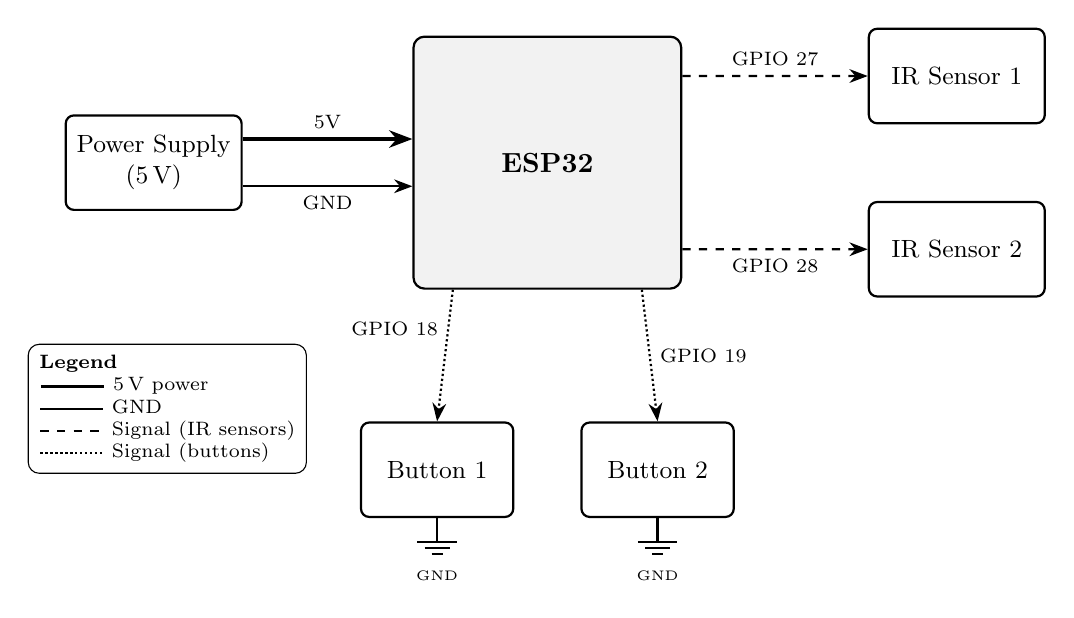
\begin{tikzpicture}
  \node[blk,text width=2.0cm] (psu) at (0,0) {Power Supply\\(5\,V)};
  \node[draw=black,fill=gray!10,thick,rounded corners=4pt,
        minimum width=3.4cm,minimum height=3.2cm,font=\bfseries] (esp) at (5,0) {ESP32};
  \node[blk,text width=2.0cm] (ir1) at (10.2,1.1)  {IR Sensor 1};
  \node[blk,text width=2.0cm] (ir2) at (10.2,-1.1) {IR Sensor 2};
  \node[blk,text width=1.7cm] (b1) at (3.6,-3.9) {Button 1};
  \node[blk,text width=1.7cm] (b2) at (6.4,-3.9) {Button 2};
  \draw[->,very thick]
     ([yshift=3mm]psu.east) -- node[above,font=\scriptsize]{5V} ([yshift=3mm]esp.west);
  \draw[->,thick]
     ([yshift=-3mm]psu.east) -- node[below,font=\scriptsize]{GND} ([yshift=-3mm]esp.west);
  \draw[->,thick,dashed]
     ([yshift=1.1cm]esp.east) -- node[above,font=\scriptsize]{GPIO 27} (ir1.west);
  \draw[->,thick,dashed]
     ([yshift=-1.1cm]esp.east) -- node[below,font=\scriptsize]{GPIO 28} (ir2.west);
  \draw[->,thick,densely dotted]
     ([xshift=-1.2cm]esp.south) -- node[left,font=\scriptsize,pos=0.3]{GPIO 18} (b1.north);
  \draw[->,thick,densely dotted]
     ([xshift=1.2cm]esp.south) -- node[right,font=\scriptsize]{GPIO 19} (b2.north);
  \gnd{b1.south}
  \gnd{b2.south}
  \node[font=\tiny,below] at ($(b1.south)+(0,-0.55)$) {GND};
  \node[font=\tiny,below] at ($(b2.south)+(0,-0.55)$) {GND};
  \node[draw,rounded corners,font=\scriptsize,align=left,anchor=north west,inner sep=4pt]
     at (-1.6,-2.3) {\textbf{Legend}\\
     \tikz[baseline=-0.5ex]\draw[very thick] (0,0)--(0.8,0);~5\,V power\\
     \tikz[baseline=-0.5ex]\draw[thick] (0,0)--(0.8,0);~GND\\
     \tikz[baseline=-0.5ex]\draw[thick,dashed] (0,0)--(0.8,0);~Signal (IR sensors)\\
     \tikz[baseline=-0.5ex]\draw[thick,densely dotted] (0,0)--(0.8,0);~Signal (buttons)};
\end{tikzpicture}}
\caption{Circuit layout of the ESP32 sensing node}
\label{fig:circuit}
\end{figure}

\subsection{Data Design}

The Firebase Realtime Database stores state as a JSON tree~\cite{firebase}. Each seat is a
leaf holding a boolean occupancy flag. Because every client subscribes to the same tree, a
single write by the ESP32 reaches all connected dashboards. Figure~\ref{fig:tree} shows the
schema and Listing~\ref{lst:json} the corresponding payload.

\begin{figure}[H]
\centering
\fitfig{%
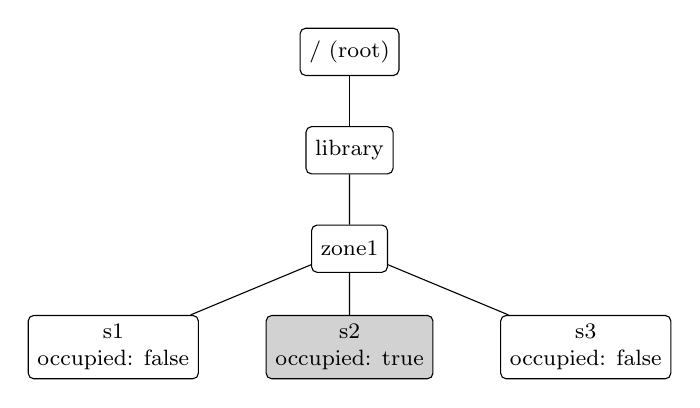
\begin{tikzpicture}[
  level distance=1.25cm,
  tn/.style={draw,rounded corners=2pt,fill=white,font=\footnotesize,minimum height=0.6cm,align=center},
  level 3/.style={sibling distance=3.0cm}]
  \node[tn] {/ (root)}
    child { node[tn] {library}
      child { node[tn] {zone1}
        child { node[tn] {s1\\occupied: false} }
        child { node[tn,fill=gray!35] {s2\\occupied: true} }
        child { node[tn] {s3\\occupied: false} }
      }
    };
\end{tikzpicture}}
\caption{JSON state-tree schema (S2 occupied, S1 and S3 vacant)}
\label{fig:tree}
\end{figure}

\Needspace{9\baselineskip}
\begin{lstlisting}[style=code,language=json,caption={Illustrative seat-state payload},label={lst:json}]
{ "library": { "zone1": {
    "s1": { "occupied": false },
    "s2": { "occupied": true  },
    "s3": { "occupied": false } } } }
\end{lstlisting}

\section{UML and Process Models}

\subsection{Use Case Diagram}

Figure~\ref{fig:usecase} shows the actors and their interactions with the system. Students use
the live seat map and entrance availability views, administrators use the analytics views, and
the sensor node detects presence and publishes state~\cite{uml}.

\begin{figure}[H]
\centering
\fitfig[0.5]{%
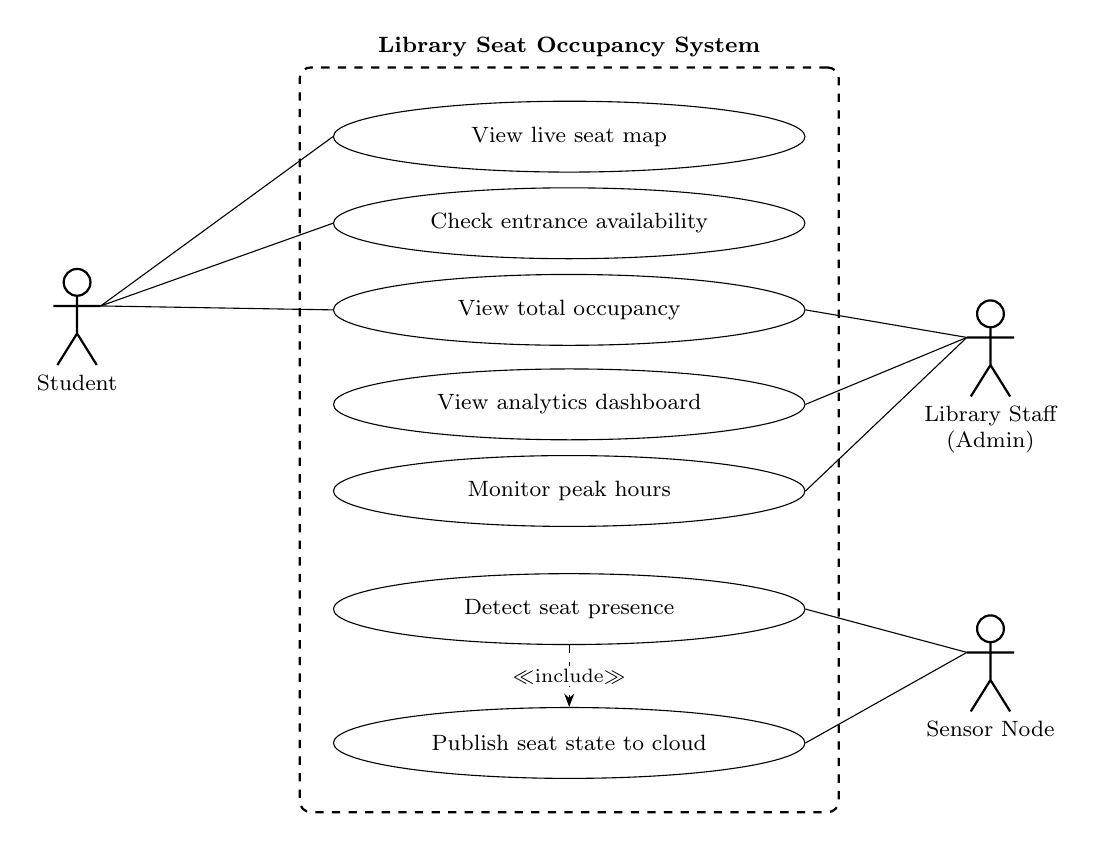
\begin{tikzpicture}[
  uc/.style={ellipse,draw,fill=white,minimum height=0.9cm,text width=4.0cm,align=center,font=\footnotesize}]
  \node[uc] (uc1) at (6.25,3.4)  {View live seat map};
  \node[uc] (uc2) at (6.25,2.3)  {Check entrance availability};
  \node[uc] (uc3) at (6.25,1.2)  {View total occupancy};
  \node[uc] (uc4) at (6.25,0)    {View analytics dashboard};
  \node[uc] (uc5) at (6.25,-1.1) {Monitor peak hours};
  \node[uc] (uc6) at (6.25,-2.6) {Detect seat presence};
  \node[uc] (uc7) at (6.25,-4.3) {Publish seat state to cloud};
  \node[draw,thick,dashed,rounded corners,fit=(uc1)(uc2)(uc3)(uc4)(uc5)(uc6)(uc7),inner sep=12pt,
        label={[font=\footnotesize\bfseries]above:Library Seat Occupancy System}] (sys) {};
  \actor{0}{1.0}{Student}
  \actor{11.6}{0.6}{Library Staff\\(Admin)}
  \actor{11.6}{-3.4}{Sensor Node}
  \draw (0.3,1.25) -- (uc1.west);
  \draw (0.3,1.25) -- (uc2.west);
  \draw (0.3,1.25) -- (uc3.west);
  \draw (11.3,0.85) -- (uc3.east);
  \draw (11.3,0.85) -- (uc4.east);
  \draw (11.3,0.85) -- (uc5.east);
  \draw (11.3,-3.15) -- (uc6.east);
  \draw (11.3,-3.15) -- (uc7.east);
  \draw[->,dashed] (uc6) -- node[fill=white,inner sep=1pt,font=\scriptsize]{$\ll$include$\gg$} (uc7);
\end{tikzpicture}}
\caption{Use case diagram}
\label{fig:usecase}
\end{figure}

\subsection{Data Flow Diagrams}

The context-level diagram (Figure~\ref{fig:dfd0}) treats the whole system as one process, and
the level-1 diagram (Figure~\ref{fig:dfd1}) decomposes it into four processes and one data
store.

\begin{figure}[H]
\centering
\fitfig[0.36]{%
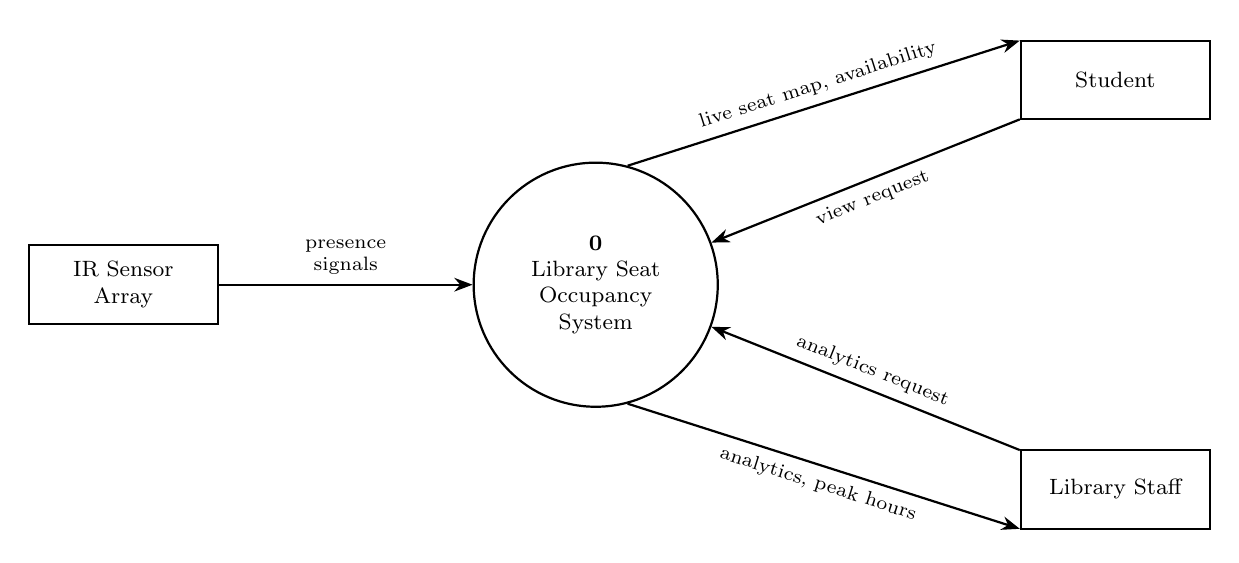
\begin{tikzpicture}[
  ent/.style={rectangle,draw,thick,fill=white,minimum width=2.4cm,minimum height=1cm,align=center,font=\footnotesize},
  proc/.style={circle,draw,thick,fill=white,minimum size=3.1cm,align=center,font=\footnotesize}]
  \node[ent]  (sens) at (0,0) {IR Sensor\\Array};
  \node[proc] (sys)  at (6,0) {\textbf{0}\\Library Seat\\Occupancy\\System};
  \node[ent]  (stud) at (12.6,2.6)  {Student};
  \node[ent]  (adm)  at (12.6,-2.6) {Library Staff};
  \draw[->,thick] (sens) -- node[fl,above]{presence\\signals} (sys);
  \draw[->,thick] (sys.75) -- node[fl,above,sloped]{live seat map, availability} ([yshift=5mm]stud.west);
  \draw[->,thick] ([yshift=-5mm]stud.west) -- node[fl,below,sloped]{view request} (sys.20);
  \draw[->,thick] (sys.-75) -- node[fl,below,sloped]{analytics, peak hours} ([yshift=-5mm]adm.west);
  \draw[->,thick] ([yshift=5mm]adm.west) -- node[fl,above,sloped]{analytics request} (sys.-20);
\end{tikzpicture}}
\caption{Data flow diagram -- level 0 (context diagram)}
\label{fig:dfd0}
\end{figure}

\begin{figure}[H]
\centering
\fitfig[0.36]{%
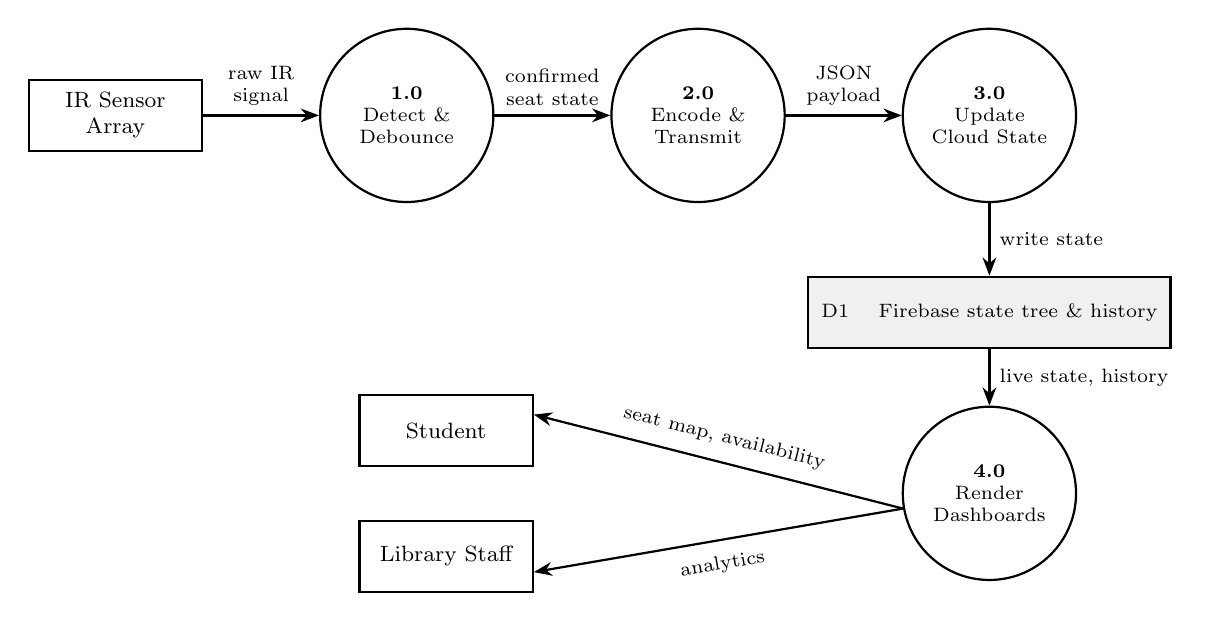
\begin{tikzpicture}[
  ent/.style={rectangle,draw,thick,fill=white,minimum width=2.2cm,minimum height=0.9cm,align=center,font=\footnotesize},
  proc/.style={circle,draw,thick,fill=white,minimum size=2.2cm,align=center,font=\scriptsize},
  store/.style={rectangle,draw,thick,fill=gray!12,minimum width=4.6cm,minimum height=0.9cm,align=center,font=\scriptsize}]
  \node[ent]  (sens) at (0,0)    {IR Sensor\\Array};
  \node[proc] (p1)   at (3.7,0)  {\textbf{1.0}\\Detect \&\\Debounce};
  \node[proc] (p2)   at (7.4,0)  {\textbf{2.0}\\Encode \&\\Transmit};
  \node[proc] (p3)   at (11.1,0) {\textbf{3.0}\\Update\\Cloud State};
  \node[store](d1)   at (11.1,-2.5) {D1 \quad Firebase state tree \& history};
  \node[proc] (p4)   at (11.1,-4.8) {\textbf{4.0}\\Render\\Dashboards};
  \node[ent]  (stud) at (4.2,-4.0)  {Student};
  \node[ent]  (adm)  at (4.2,-5.6)  {Library Staff};
  \draw[->,thick] (sens) -- node[fl,above]{raw IR\\signal} (p1);
  \draw[->,thick] (p1) -- node[fl,above]{confirmed\\seat state} (p2);
  \draw[->,thick] (p2) -- node[fl,above]{JSON\\payload} (p3);
  \draw[->,thick] (p3) -- node[fl,right]{write state} (d1);
  \draw[->,thick] (d1) -- node[fl,right]{live state, history} (p4);
  \draw[->,thick] (p4.190) -- node[fl,above=2pt,sloped]{seat map, availability} ([yshift=2mm]stud.east);
  \draw[->,thick] (p4.-170) -- node[fl,below=2pt,sloped]{analytics} ([yshift=-2mm]adm.east);
\end{tikzpicture}}
\caption{Data flow diagram -- level 1}
\label{fig:dfd1}
\end{figure}

\subsection{Behavioural Models}

\textbf{Sequence diagram.} 
Figure~\ref{fig:seq} follows one seat-occupancy event from a student sitting down to the seat
turning red on every connected dashboard.

\begin{figure}[H]
\centering
\fitfig[0.36]{%
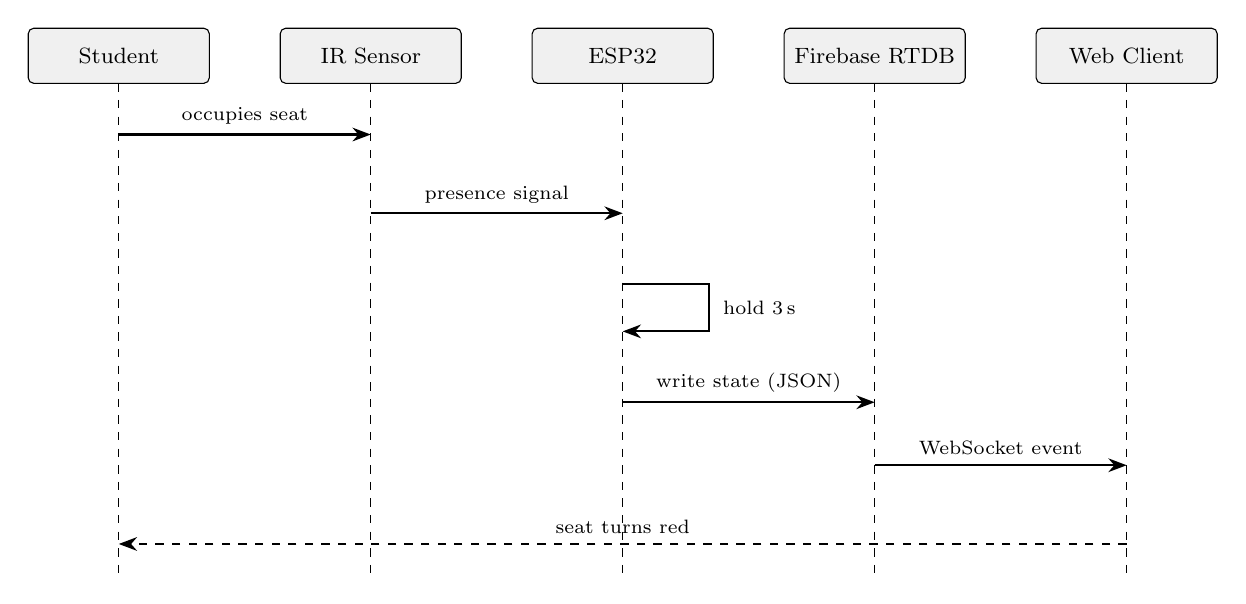
\begin{tikzpicture}[x=1cm,y=1cm]
  \foreach \x/\n in {0/Student,3.2/IR Sensor,6.4/ESP32,9.6/Firebase RTDB,12.8/Web Client}{
    \node[draw,fill=gray!12,rounded corners=2pt,minimum width=2.3cm,minimum height=0.7cm,font=\footnotesize] at (\x,0) {\n};
    \draw[dashed] (\x,-0.35) -- (\x,-6.6);
  }
  \draw[->,thick] (0,-1.0)   -- node[above,font=\scriptsize]{occupies seat} (3.2,-1.0);
  \draw[->,thick] (3.2,-2.0) -- node[above,font=\scriptsize]{presence signal} (6.4,-2.0);
  \draw[->,thick] (6.4,-2.9) -- (7.5,-2.9) -- (7.5,-3.5) -- (6.4,-3.5);
  \node[font=\scriptsize,right] at (7.55,-3.2) {hold 3\,s};
  \draw[->,thick] (6.4,-4.4) -- node[above,font=\scriptsize]{write state (JSON)} (9.6,-4.4);
  \draw[->,thick] (9.6,-5.2) -- node[above,font=\scriptsize]{WebSocket event} (12.8,-5.2);
  \draw[->,thick,dashed] (12.8,-6.2) -- node[above,font=\scriptsize]{seat turns red} (0,-6.2);
\end{tikzpicture}}
\caption{Sequence diagram for a seat-occupancy event}
\label{fig:seq}
\end{figure}

\textbf{Seat state machine.} Each seat is modelled as the four-state machine in Figure~\ref{fig:fsm}. A seat changes
between \textsc{Vacant} and \textsc{Occupied} only after the new reading has been stable for
3~seconds; a shorter disturbance returns it to the previous confirmed state (dashed
transitions).

\begin{figure}[H]
\centering
\fitfig[0.36]{%
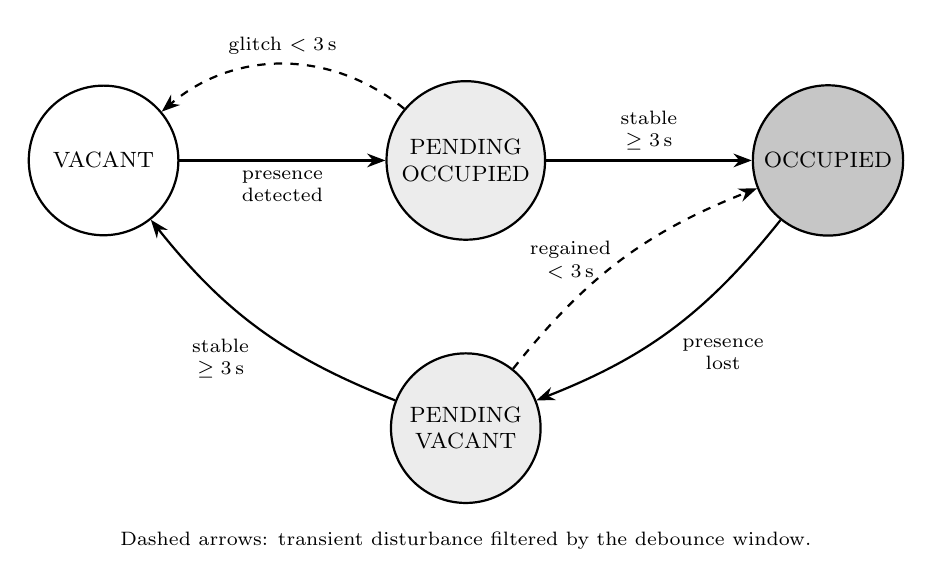
\begin{tikzpicture}[
  st/.style={circle,draw,thick,minimum size=1.9cm,align=center,font=\footnotesize}]
  \node[st,fill=white] (v)  at (0,0)     {VACANT};
  \node[st,fill=gray!15] (p1) at (4.6,0)  {PENDING\\OCCUPIED};
  \node[st,fill=gray!45] (o)  at (9.2,0)   {OCCUPIED};
  \node[st,fill=gray!15] (p2) at (4.6,-3.4) {PENDING\\VACANT};
  \draw[->,thick] (v) -- node[fl,below]{presence\\detected} (p1);
  \draw[->,thick] (p1) -- node[fl,above]{stable\\$\geq 3$\,s} (o);
  \draw[->,thick] (o) to[bend left=15] node[fl,below right]{presence\\lost} (p2);
  \draw[->,thick] (p2) to[bend left=15] node[fl,below left]{stable\\$\geq 3$\,s} (v);
  \draw[->,thick,dashed] (p1) to[bend right=40] node[fl,above]{glitch $<3$\,s} (v);
  \draw[->,thick,dashed] (p2) to[bend left=15] node[fl,left,pos=0.5]{regained\\$<3$\,s} (o);
  \node[fl,anchor=north] at (4.6,-4.6) {Dashed arrows: transient disturbance filtered by the debounce window.};
\end{tikzpicture}}
\caption{Seat state machine with 3-second debounce}
\label{fig:fsm}
\end{figure}

\textbf{Firmware flowchart.} The main loop of the ESP32 firmware is shown in Figure~\ref{fig:flow}.

\begin{figure}[H]
\centering
\fitfig[0.42]{%
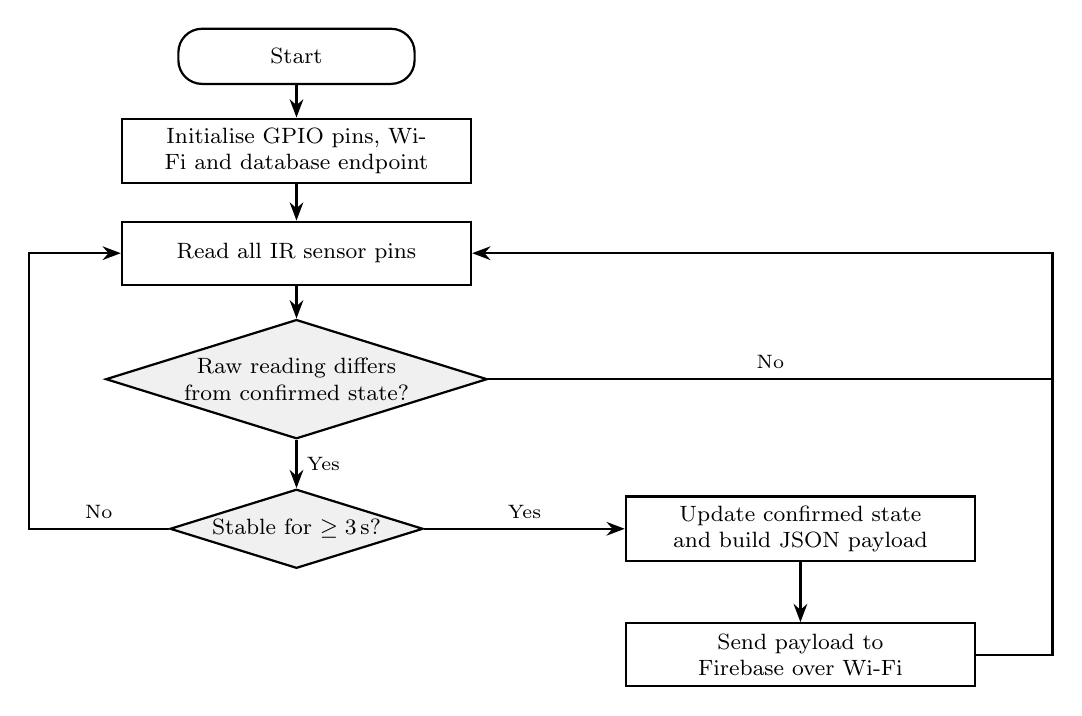
\begin{tikzpicture}[
  term/.style={rectangle,rounded corners=0.3cm,draw,thick,fill=white,minimum height=0.7cm,minimum width=3cm,font=\footnotesize,align=center},
  prc/.style={rectangle,draw,thick,fill=white,minimum height=0.8cm,text width=4.2cm,font=\footnotesize,align=center},
  dec/.style={diamond,aspect=3.2,draw,thick,fill=gray!12,inner sep=1pt,font=\footnotesize,align=center}]
  \node[term] (start) at (0,0)    {Start};
  \node[prc]  (init)  at (0,-1.2) {Initialise GPIO pins, Wi-Fi and database endpoint};
  \node[prc]  (read)  at (0,-2.5) {Read all IR sensor pins};
  \node[dec]  (d1)    at (0,-4.1) {Raw reading differs\\from confirmed state?};
  \node[dec]  (d2)    at (0,-6.0) {Stable for $\geq 3$\,s?};
  \node[prc]  (upd)   at (6.4,-6.0) {Update confirmed state and build JSON payload};
  \node[prc]  (send)  at (6.4,-7.6) {Send payload to Firebase over Wi-Fi};
  \draw[->,thick] (start) -- (init);
  \draw[->,thick] (init) -- (read);
  \draw[->,thick] (read) -- (d1);
  \draw[->,thick] (d1) -- node[right,font=\scriptsize]{Yes} (d2);
  \draw[->,thick] (d2) -- node[above,font=\scriptsize]{Yes} (upd);
  \draw[->,thick] (upd) -- (send);
  % loop back to the sensor-reading step (right side)
  \draw[thick] (d1.east) -- node[above,font=\scriptsize]{No} (9.6,-4.1);
  \draw[thick] (send.east) -- (9.6,-7.6) -- (9.6,-4.1);
  \draw[->,thick] (9.6,-4.1) -- (9.6,-2.5) -- (read.east);
  % loop back (left side) when the reading is not yet stable
  \draw[->,thick] (d2.west) -- node[above,font=\scriptsize]{No} (-3.4,-6.0) -- (-3.4,-2.5) -- (read.west);
\end{tikzpicture}}
\caption{Firmware main-loop flowchart}
\label{fig:flow}
\end{figure}

\section{Implementation Details}

\subsection{Firmware (ESP32)}
% (ESP32)}

The firmware polls the IR pins, applies the 3-second debounce per seat and publishes the
confirmed states as JSON. Listing~\ref{lst:fw} is an illustrative implementation of this
logic; pin numbers follow Figure~\ref{fig:circuit}.

\Needspace{17\baselineskip}
\begin{lstlisting}[style=code,language=C++,caption={Illustrative firmware logic for debounce and publishing},label={lst:fw}]
constexpr uint32_t DEBOUNCE_MS = 3000;   // 3-second debounce window
struct Seat { uint8_t pin; bool confirmed, candidate; uint32_t changedAt; };
Seat seats[2] = { {27, false, false, 0}, {28, false, false, 0} };

void publishState() {                    // build JSON and write once
  String json = "{";
  for (int i = 0; i < 2; ++i) {
    json += "\"s" + String(i + 1) + "\":{\"occupied\":";
    json += seats[i].confirmed ? "true}" : "false}";
    if (i < 1) json += ",";
  }
  json += "}";
  HTTPClient http;  http.begin(DB_URL);
  http.PUT(json);   http.end();          // clients notified by the database
}
void loop() {
  bool dirty = false;
  for (auto &s : seats) {
    bool raw = (digitalRead(s.pin) == LOW);         // active-low IR module
    if (raw != s.candidate) { s.candidate = raw; s.changedAt = millis(); }
    if (s.candidate != s.confirmed && millis() - s.changedAt >= DEBOUNCE_MS) {
      s.confirmed = s.candidate;  dirty = true;
    }
  }
  if (dirty) publishState();
}
\end{lstlisting}

\subsection{Cloud Layer and Web Application}

The Firebase Realtime Database holds the state tree of Figure~\ref{fig:tree}. Clients attach
listeners to the tree and receive updates as events over a persistent WebSocket connection, so
no polling is required.

The web application is built with React~\cite{react} and branded \emph{SmartLib}. It has a
\emph{Student} view and an \emph{Admin} view, reachable from the navigation bar. The floor map
is made of SVG nodes whose fill colour is bound to each seat's occupancy flag, so a database
update re-renders the affected seat immediately.

\textbf{Student dashboard.} Shows live capacity metrics and the seat layout. Summary cards
report total, occupied and available seats and the occupancy rate (in the example shown: 4
seats, 2 occupied, 2 available, 50\%). A seat-layout panel shows seats S01--S04 around a study
table; available seats are green and occupied seats are red.

\textbf{Admin dashboard.} Provides utilisation analytics. Summary cards report total seats,
occupied seats, average session time and the peak hour. A weekly occupancy trend, an hourly
peak-hours histogram and a donut chart of the available/occupied split support traffic
balancing and facility planning.

\textbf{Entrance kiosk.} The same application shows live capacity at the library gate.

% ===== CHAPTER 3: RESULTS & EVALUATION =====

\chapter{Results and Evaluation}
\label{ch:results}

\section{Testing Methodology}

The planned test cases in Table~\ref{tab:tests} verify the functional and non-functional
requirements of Chapter~\ref{ch:method}.

\begin{table}[H]
\centering
\footnotesize
\renewcommand{\arraystretch}{1.0}
\begin{tabularx}{\linewidth}{|l|>{\raggedright\arraybackslash}p{0.34\linewidth}|X|l|}
  \hline
  \textbf{ID} & \textbf{Scenario} & \textbf{Expected outcome} & \textbf{Req.} \\
  \hline
  T1 & A person occupies a vacant seat & After the 3-s debounce the seat turns red on all
       dashboards & FR1, FR2, FR5 \\
  \hline
  T2 & The person leaves the seat & After 3\,s the seat turns green & FR1, FR2, FR5 \\
  \hline
  T3 & A hand or bag passes the sensor for less than 3\,s & No state change is published
       & FR2, NFR2 \\
  \hline
  T4 & Two clients are open simultaneously & Both update from the same database event
       without refresh & FR4 \\
  \hline
  T5 & Occupancy counts are inspected & Occupied $+$ available equals total seats; the
       rate is correct & FR6 \\
  \hline
  T6 & The Wi-Fi connection drops and returns & The node resumes publishing and dashboards
       show the current state & NFR1 \\
  \hline
  T7 & The kiosk page is opened at the gate & Live capacity matches the student dashboard
       & FR7 \\
  \hline
  T8 & Admin dashboard is opened & Session time, peak hour and charts are displayed & FR8 \\
  \hline
\end{tabularx}
\caption{Test cases and expected outcomes}
\label{tab:tests}
\end{table}

\section{Analysis}

The prototype demonstrates the complete data path: an IR sensor feeding an ESP32 node, a JSON
state in a cloud database, and browser dashboards updated through WebSocket events. Seat-level
sensing removes the main weakness of gate counters, and the 3-second debounce keeps the colour
indicators stable.

\subsection{Limitations}

An IR sensor detects an obstruction, not a person, so an object left on a desk can be reported
as occupied. The system depends on library Wi-Fi and the cloud service, and larger deployments
need more nodes, pin and power planning and sensor calibration.

% ===== CHAPTER 4: CONCLUSION =====

\chapter{Conclusion}
\label{ch:concl}

\section{Summary of Work}

This project delivers a working architecture for a real-time, seat-level library occupancy
system built from low-cost IoT hardware and a reactive cloud stack. It addresses the three
identified problems: it reduces manual searching by showing free seats remotely, replaces
aggregate gate counts with micro-level desk availability, and gives administrators live and
historical analytics.

\section{Future Work and Recommendations}

\begin{enumerate}
  \item Combine IR with a second sensing modality to distinguish a person from an object.
  \item Add seat reservation and time-limited holds.
  \item Forecast occupancy from the stored history to predict peak hours.
  \item Adopt a lightweight messaging protocol such as MQTT and battery or low-power operation.
  \item Extend to multi-zone and multi-floor deployment with a campus-wide map.
  \item Send push notifications when a preferred seat or zone becomes free.
\end{enumerate}

% ===== BIBLIOGRAPHY =====

% Entries not cited in the text are still listed
\nocite{pressman,sommerville}

\clearpage
\phantomsection
\addcontentsline{toc}{chapter}{Bibliography}
\begin{thebibliography}{BRJ05}
\bibitem[BRJ05]{uml} Grady Booch, James Rumbaugh, and Ivar Jacobson. \emph{The Unified Modeling Language User Guide}. 2nd ed. Addison-Wesley, 2005.
\bibitem[Esp]{esp32} Espressif Systems. \emph{ESP32 Series Datasheet}. Espressif Systems. \url{https://www.espressif.com}.
\bibitem[Goo]{firebase} Google. \emph{Firebase Realtime Database Documentation}. \url{https://firebase.google.com/docs/database}.
\bibitem[Met]{react} Meta Open Source. \emph{React Documentation}. \url{https://react.dev}.
\bibitem[PM19]{pressman} Roger S. Pressman and Bruce R. Maxim. \emph{Software Engineering: A Practitioner's Approach}. 9th ed. McGraw-Hill, 2019.
\bibitem[Som16]{sommerville} Ian Sommerville. \emph{Software Engineering}. 10th ed. Pearson, 2016.
\end{thebibliography}

\end{document}
